\chapter{Tests and Validation}\label{chap:tests}

Some of the tests made during the exploration have already been mentioned in
\autoref{chap:expl}, but here we will go over a couple of tests in detail that
were important in the development of our tool and verifying that it worked as
expected.

\section{Validation in Emulated Environment}

After developing the initial version of the full service program, one of the
tests we performed using Mininet-WiFi consisted of three stations (named sta1
sta2 and sta3), where sta1 and sta3 were too far apart from each other to
communicate directly, but both in range of sta2, as shown in
\autoref{fig:latetest}, and all of them without any paths in their mesh path
tables initially, pinging sta3 from sta1. The host system used the Arch Linux
distribution, running the \ac{LTS} version 5.10 Linux kernel.

\begin{figure}[htb]
   \centering
   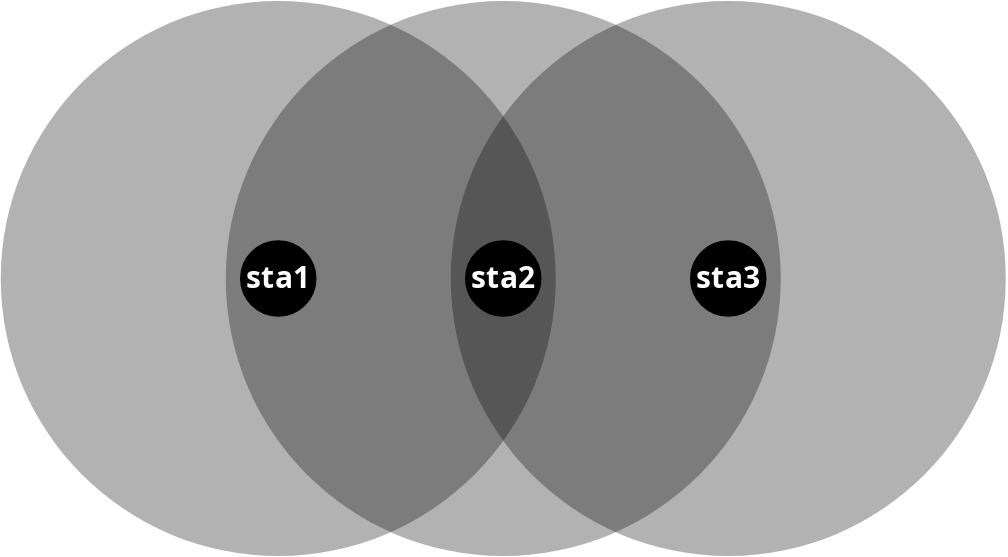
\includegraphics[scale=.3]{latetest}
   \caption{Test configuration used in Mininet-WiFi}\label{fig:latetest}
\end{figure}

We found that the first station to create and add a mesh path was sta3. Although
sta1 was the one that pinged sta3, it could not create a path yet because it did
not know the \ac{MAC} address of sta3. So sta1 only sends an \ac{ARP} request in
broadcast, which is then retransmitted by sta2, and after sta3 receives it, it
creates a path for sta1 (without the nexthop field filled in) when it sends its
\ac{ARP} response, highlighted in blue in \autoref{fig:capsta3}, which shows the
packet capture that was executed in sta3.

\begin{figure}[htb]
   \centering
   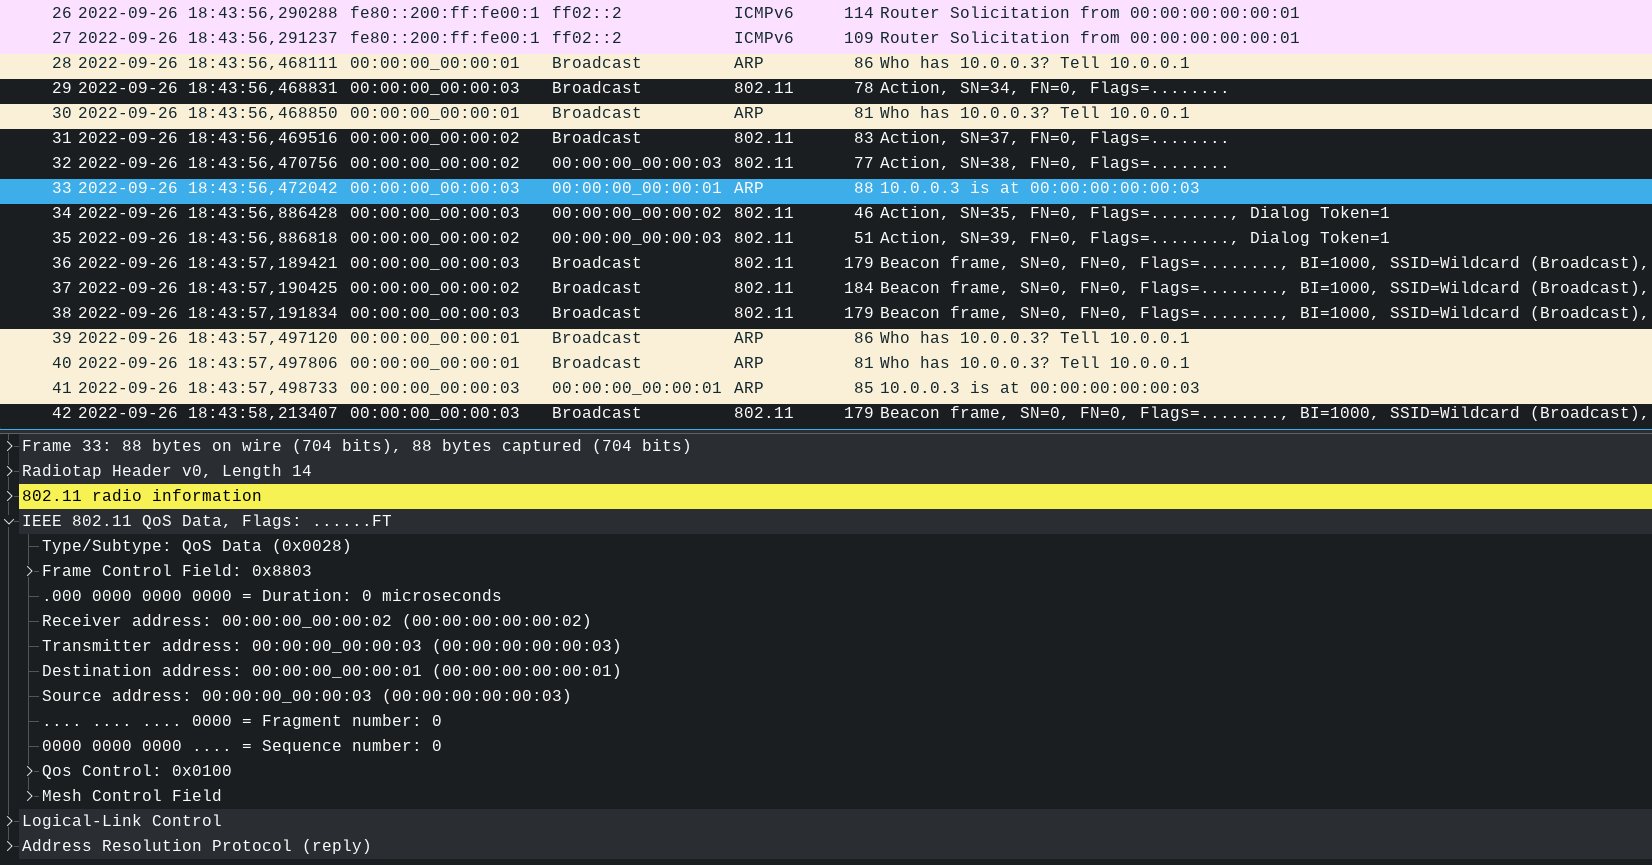
\includegraphics[scale=.35]{capsta3}
   \caption{\ac{ARP} response that caused a path to be added to the mesh path table}\label{fig:capsta3}
\end{figure}

Immediately after, sta2 creates a path to sta3 and retransmits the \ac{ARP}
response to sta1, which in turn receives the \ac{MAC} address of sta3 through
sta2, and creates its mesh paths, both for sta2 and sta3.


\section{Validation with Hardware Nodes}\label{sect:valid}

Because we spent most of our time in development testing with Mininet-WiFi, we
were only able to do a simple test with real hardware, using two computers
running Arch Linux, just like the host system used in the tests in the emulated
environment (one using the \texttt{rtl8723be} driver for the wireless network
controller and the other using \texttt{iwlwifi}), and a third computer running
Fedora 36 with version 5.17 of the Linux kernel, also using the \texttt{iwlwifi}
driver. We tried to replicate the test mentioned in the previous section,
placing sta1 and sta3 far away from each other in the hopes that sta2 would be
needed for the other two stations to communicate, but the space we had was not
enough, as can be seen in the results displayed in \autoref{fig:hardtest}, which
shows at the bottom details about the first event captured in sta3, where a path
was added with the destination and the nexthop both set to sta1's \ac{MAC}
address, meaning sta2 was not used for communication between the two stations.
Still, we can verify that the tool we developed worked as expected, showing a
mesh path being created and then deleted in sta2 (most likely because it ended
up not being used), and sta3 and sta1 creating mesh paths and settings their
\textbf{nexthops} values.

We did notice some unexpected behaviour. For example, in event number 10, sta1
changed the \textbf{nexthop} field of its path to sta3 to the value it already
had previously, effectively not changing anything. The reason for this behaviour
was most likely a change to the path's sequence number, which is a field we do
not capture, but is maintained in the mesh path table entries.
